% Chapter 4 from the standard thesis template
% that contains an adv. example table and figure.
\chapter{SOFTWARE DEFINED RADIOMETER IMPLEMENTATION}\label{ch:implementation}

This chapter examines the implementation of a software defined radio based radiometer.  This requires that we understand the requirements of both a traditional radiometer and a digital radiometer which we will examine in this chapter.  Next we will map the traditional radiometer components discussed in chapter \ref{ch:background} to their digital counterparts.  Finally we will give an overview of the software defined radiometer implemented in this thesis.

\section{Requirements}\label{requirements}

This section discusses the hardware and software requirements used to drive the selection of the hardware and software platforms use to implement our software defined radio based radiometer.  

\emph{Hardware Requirements.}  The capabilities of existing traditional radiometers were the primary driving force in setting the requirements of our hardware development platform.  Dr. Brian Hornbuckle from the ECE and Agronomy department at Iowa State University was consulted with respect to key specifications of his radiometer.  Additionally, the specifications of other radiometers were examined. 

Table \ref{rad_performance} summarizes the specification of three parameters that were decided upon for selecting our hardware development platform, based on our investigation.  This lead to the the selection of the N200 software defined radio platform with a DBSRX2 daughter board from Ettus Research as our platform.  Section \ref{SDR_platform} provides more in depth information on the hardware used and why it was selected.

\begin{table}[h!tb] \centering
\isucaption{Required Radiometer performance}
\label{rad_performance}
% Use: \begin{tabular{|lcc|} to put table in a box
\begin{tabular}{lcc} \hline
\textbf{Parameter} & \textbf{Value} & \textbf{Units} \\ \hline
Minimum bandwidth & 20 & MHz \\
Operational frequency & 1400 - 1420 & MHz \\
$NE\Delta T$ & 1 & Kelvin \\ \hline
\end{tabular}
\end{table}

\emph{Software Requirements.}  Since an objective of this work was to help make radiometers more wildly accessible to the general research and education communities, a requirement of the development software was ease of use.  Additionally, the user interfaces developed with these software tools needed to be easy to use, while providing sufficient computing efficiency for the signal processing required for radiometry.

GNURadio met the stated requirements.  It includes a supplemental software package called GNURadio Companion (GRC), which uses a graphical interface for creating a radio environment.  GNURadio and GRC are discussed in greater detail in Section \ref{software_platform}.

%Since an easy to use system was a requirement in the selection of the software.  GNURadio was selected as it includes GNURadio Companion (GRC), a supplemental program which uses a graphical interface for creating the radio environment.  GNURadio and GRC is discussed in greater detail in Chapter \ref{ch:background}, section \ref{software_platform}. 

\section{Mapping Traditional Radiometer Functions to a Software Defined Radio Radiometer}

The use of a software defined radio (SDR) to implement a radiometer requires mapping components of a traditional radiometer to SDR-based technology.  This section presents the mapping of three such components for implementing our SDR-based radiometer.  These components are:  1) power measurement, 2) integration, and 3) filtering.

\subsection{Power measurement}

A traditional radiometer uses a device called a square law detector to measure power.  It transforms an input signal into an output voltage whose square is proportional to the input signal power.  For a signal that is the thermal noise of the object, the mean value is zero.  However, a square-law detector takes the peak values of the envelope of the signal.  This is shown in Figure ....


{\begin{figure}[h!tb] 
\centering
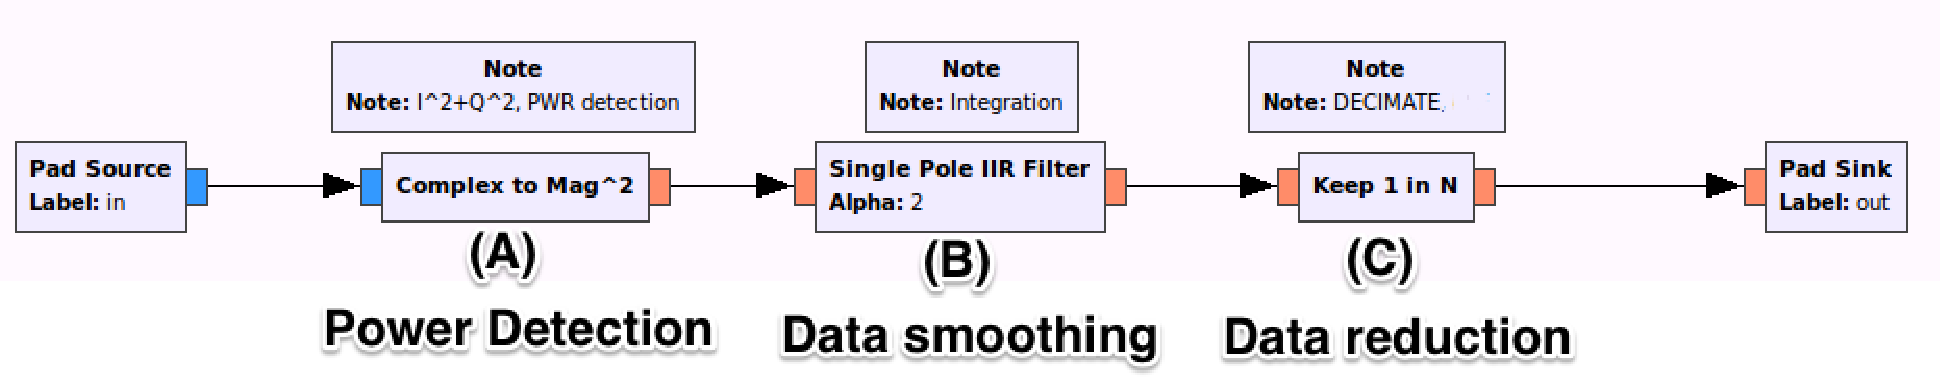
\includegraphics[width=17cm]{Images/TPR_grc.png}
\isucaption{A block diagram showing how the radiometer performs the equivalent square law detector in software.}
\label{square_block}
\end{figure}
}

Equation \ref{sdr_x2} gives the mathematical representation of a square law detector's functionality where I is the in-phase of the input signal, Q is the quadrature-phase of the input signal, and $P_{out}$ is the power of the signal.

To implement this in software, a square law detector is built mathematically as the sum of the squares[\cite{Sarijari}].  Once a signal has been digitized, it is expressed in data bits of I and Q, which represent the in-phase and the quadrature-phase of the signal.  By squaring each term, we get the desired result of the power of the signal and this is shown in equation \ref{sdr_x2}[\cite{Rashid}].

\begin{equation}\label{sdr_x2}
I^2+Q^2 = P_{out}
\end{equation}

Like the analog square-law detector we are taking peak voltage values, which has an equivalent noise voltage and a mean value of zero, and square them to produce a noise power that is proportional to the square of this amplitude.  Figure \ref{square_block} shows the GNURadio blocks used to perform this function.

Like the analog square-law detector, this signal will fluctuate rapidly.  To improve the sensitivity of the radiometer the signal is integrated.  The next step is to replicate a RC filter or integrator in the software defined radio.

\subsection{Integration}

To improve our sensitivity, and reduce the rapid fluctuations in the power measurements, we integrate the power measurements.  This gives an average of the signal and reduces the fluctuations in the output.  This helps to improve the sensitivity of the radiometer as seen in equation \ref{NEAT_EQ}.  The digital equivalent to a integrator is a Finite Impulse Response (FIR) filter.

A FIR filter is a digital filter that can take an impulse signal and decays to zero after a finite number of iterations.  This type of digital filter can be represented by equation \ref{FIR_Eq} which mathematically expresses the FIR Filter and simply says that the nth output is a weighted average of the most recent P inputs. 

\begin{equation}\label{FIR_Eq}
y_n=\displaystyle\sum\limits_{i=o}^{P-1} c_ix_{n-i}
\end{equation} 

An Infinite Impulse Response (IIR) filter is the same as the FIR filter, except a summation term is added which feeds back the previous output.  Equation \ref{IIR_eq} shows that a FIR filter is a IIR filter, except $Q=0$[\cite{Cross}]. 

\begin{equation}\label{IIR_eq}
y_n=\displaystyle\sum\limits_{i=o}^{P-1} c_ix_{n-i}+\displaystyle\sum\limits_{j=1}^{Q} d_jy_{n-j}
\end{equation}

Both filters produce the same result by giving the average of the input signal.  An IIR filter however uses less computational power than a FIR filter.  Because of this, an IIR filter was used in defining our integrator in a software defined radiometer.

To get a better understanding on how the digital IIR filter relates to the RC filter analog, look at the Fourier Transform and the relationship of the input to the output in the frequency domain in equation \ref{Fourier_IIR}.  In equation \ref{Fourier_IIR}, $f$ is our frequency in Hz and $T$ is the time between samples in seconds and is related to our sampling frequency.

\begin{equation}\label{Fourier_IIR}
H(f)=\frac{\displaystyle\sum\limits_{j=o}^{P-1} c_je^{-2\pi ijfT}}{1-\displaystyle\sum\limits_{k=1}^{Q} d_ke^{-2\pi ikfT}}
\end{equation}

Now to show the link between the analog RC circuit and the IIR filter we look at equation \ref{eq:rc_circuit_eq}.  

\begin{equation}\label{eq:rc_circuit_eq}
\frac{V_{in}-V_{out}}{R}=C\frac{dV_{out}}{dt}
\end{equation}

Equation \ref{eq:rc_circuit_eq} represents the differential equation relating the input voltage $V_{in}$ to the output voltage $V_{out}$.  We can substitute for input and output of our IIR filter in terms of $x_n$ and $y_n$.  Because we are now in the time domain, we need to define what $T$ is and we can do that using equation \ref{sampling_rate_eq}.

\begin{equation}\label{sampling_rate_eq}
T=time between samples=\frac{1}{sampling rate}
\end{equation}

We can now relate our input voltage to the input to our IIR filter shown in equation \ref{input_IIR} and the output voltage shown in equation \ref{output_IIR}.

\begin{equation}\label{input_IIR}
x_n=v_{in}(nT)
\end{equation}

\begin{equation}\label{output_IIR}
y_n=v_{out}(nT)
\end{equation}

Next we rewrite our difference equation with $x_n$ and $y_n$ shown in equation \ref{diff_xn_yn}.

\begin{equation}\label{diff_xn_yn}
\frac{x_n-y_n}{R}=C\frac{y_n-y_{n-1}}{T}
\end{equation}

Finally, we can solve for $y_n$ which results in our final equation \ref{final_IIR_RC}.

\begin{equation}\label{final_IIR_RC}
y_n=\frac{T}{T+RC}x_n+\frac{RC}{T+RC}y_{n-1}
\end{equation}

It can be seen that an IIR filter can have the same frequency response as we expect from an analog RC filter.  As our sampling rate approaches infinity, the approximation gets closer to the original response from the analog RC circuit.  

%The $RC$ term gives us our time constant of the circuit and can be used to calculate out our coefficients.  We are not concerned about the actual values of R and C with our IIR filter, instead we just need the product of R and C.  

In GNURadio most of the work is done for us.  We can simply enter in our desired cutoff frequency and GNURadio will calculate our IIR filter coefficients.  However, this shows that an IIR filter works much like an analog RC low pass filter.

\subsection{Bandwidth and filtering}
A traditional radiometer will use filters to restrict the bandwidth of the radiometer.  For a software defined radiometer, the sampling rate defines the bandwidth for a software defined radiometer.  

Additional filtering can be created and used in a software defined radiometer.  These filters are often created using either IIR or FIR filters.  The most efficient method is to restrict bandwidth by setting the sampling rate.  However, these filters can be used to filter out a narrow band of frequencies.  This will be discussed in chapter \ref{ch:results}.

\section{System overview}

Like a traditional radiometer, the SDR uses an antenna to look at the target of interest.  SDRs still use an amplification to improve the sensitivity of the SDR. After that stage though, a software defined radiometer is different.  A SDR will sample and generate I and Q values that represents the signal.  From there, this data is sent to a computer to be processed.  We can then use this information to calculate the power of the signal.  In addition, we can manipulate the signal in other ways such as applying a filter to filter out an unwanted source.

%As we have shown the two of the major components of a traditional radiometer, the power detection and integration of the signal can be replicated in software and therefore can be implemented in a software defined radio.  The information can now be stored, displayed or both for further analysis.  

%There is one component of the software defined radio that we are not able to implement in software and that is with the signal amplification.  This however does play a major role in the performance of the radiometer and is a key element that should not be overlooked.  While this is not implemented in software, it still plays a critical role in our software defined radio radiometer. 

Next we will now look at how we control the software defined radiometer using the software detailed in chapter \ref{ch:background}, section \ref{software_platform} in defining the radiometer.  We will also look at how the data is displayed and stored in the software defined radiometer.

\subsection{Control of the SDR Hardware through GNURadio}
The N200 sends all data across the 1 Gbps Ethernet connection to be read in by a host computer running GNURadio.  This data is the raw I/Q values that is read by the on board A/D and processed by the on board FPGA.  An example of a very simple GNURadio software implementation would simply take this data and store the data to a hard drive in a file.  This can be very handy if we want to simply record the data and then process it later.  However, depending on the sample rate, this can consume a large amount of storage.  A short recording can  consume 1-2 GB with a sample rate of 10 Msps.  This simple system also does not give us any immediate feedback on the radiometer and it does not give us controls of the radiometer such as frequency, integration time or other key variables.  Fortunately GNURadio has tools that allows us to build up a very rich application that is able to give us the data we need and control the software defined radio as well.

The GNURadio Companion allows us to create python code that is used to not only receive the data from the SDR but also perform signal processing on the incoming information.  Additional controls are added that allow for tuning of the signal processing parameters and control of the radio functions.  With this we can build up an application that can be run on any computer that is capable of running GNURadio.  

{\begin{figure}[h!tb] 
\centering
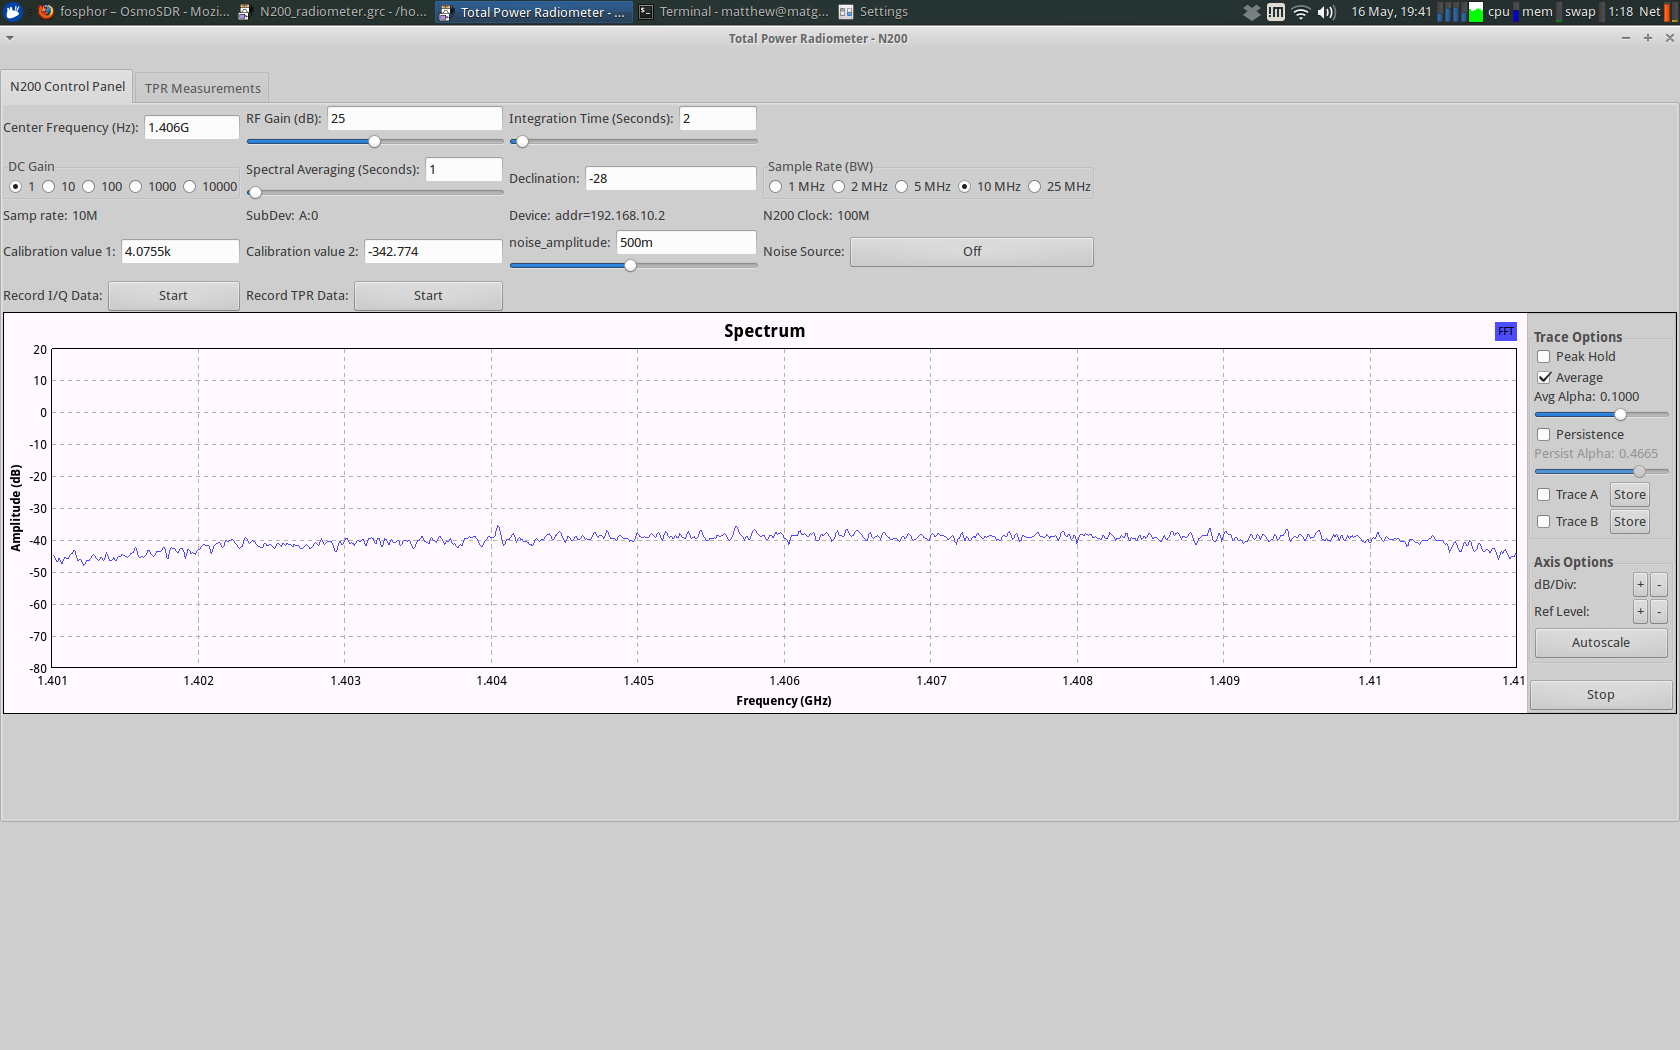
\includegraphics[width=17cm]{Images/radiometer_gui.png}
\isucaption{A screenshot of the interface made for communication with and controlling the software defined radio}
\label{radiometer_gui}
\end{figure}
}

Through this interface we are able to control several key aspects of the radio hardware within the SDR.  This has the impact of affecting the behavior of this software defined radiometer as well.  Through this we can control: frequency, sample rate (Bandwidth), integration time, and the gain on the DBSRX2 daughter board.  We will no look at how these controls impact the performance of the radiometer.  

\subsection{Impact of the Controls Related to Radiometry}

Having the ability to control these key aspects of the software defined radiometer allows us to affect the performance of the radiometer.  The $NE\Delta T$, equation \ref{NEAT_EQ}, discussed in chapter \ref{ch:background} outlines what some of these changes affect in a radiometer.

%For any radiometer noise temperature is a large consideration and is critical to the design of the radiometer.  One method to determine how well a radiometer is to look at the sensitivity of the radiometer.  We can do this by looking at the smallest change in temperature the radiometer can see.  We will call this the Noise Equivalent $\Delta T$ or $NE\Delta T$ of the radiometer and is equation \ref{NEAT_EQ} covered in chapter \ref{ch:background}.

$\beta$ can be changed by changing the sample rate of the SDR.  The sample rate effectively controls the bandwidth in which the SDR is operating at.  This also gives us a band-pass filter as well, since the SDR will not respond to frequencies outside of this bandwidth.  

$\tau$ is the integration time for the radiometer.  This parameter is set by the user through the GUI and allows us to change the integration time in seconds.

We will now look at how this data is handled and displayed by the software defined radiometer.

\subsection{GNURadio Data Handling}
Once we have the data that has been processed by the software defined radio we will want to display this information and be able to store the data so we can analyze it later if needed.  Data display is handled by GNURadio by plotting the total power over time.  This allows the user to be able to visualize the total power and be able to determine if the total power has increased or decreased over the time window shown.  

We also have the ability to look at a signal in terms of frequency versus amplitude.  This allows looking for any unusual signals that may be interfering with the system or causing erroneous data with our radiometer and is covered in chapter \ref{ch:results}.  

Finally, we will want to store the data so we can do additional analyses on it at a later time.  The GNURadio program allows us to store the data in two formats.  The first format is storing the raw I/Q data from the radiometer.  This format allows us to playback the data through GNURadio at a later time.  This can be useful for if we wish to change parameters in GNURadio such as bandwidth or integration time.  It is also a good diagnostic tool as we can check that the signal coming in is clean or if we need to apply additional filters to remove an unwanted signal.

The second format is the total power that has been calculated by the radiometer.  This file is much smaller since much of the signal information has now been reduced to simple power versus time information.  This allows for easy manipulation through any math program such as Matlab for analysis.  

\subsection{GNURadio Data Display}
The information from the software defined radio can be displayed through GNURadio to show a number of things.  Since we have both frequency and magnitude information we can display this information.  We are able to also display the information that shows the total power that is being seen by the radiometer as well.

{\begin{figure}[h!tb] 
\centering
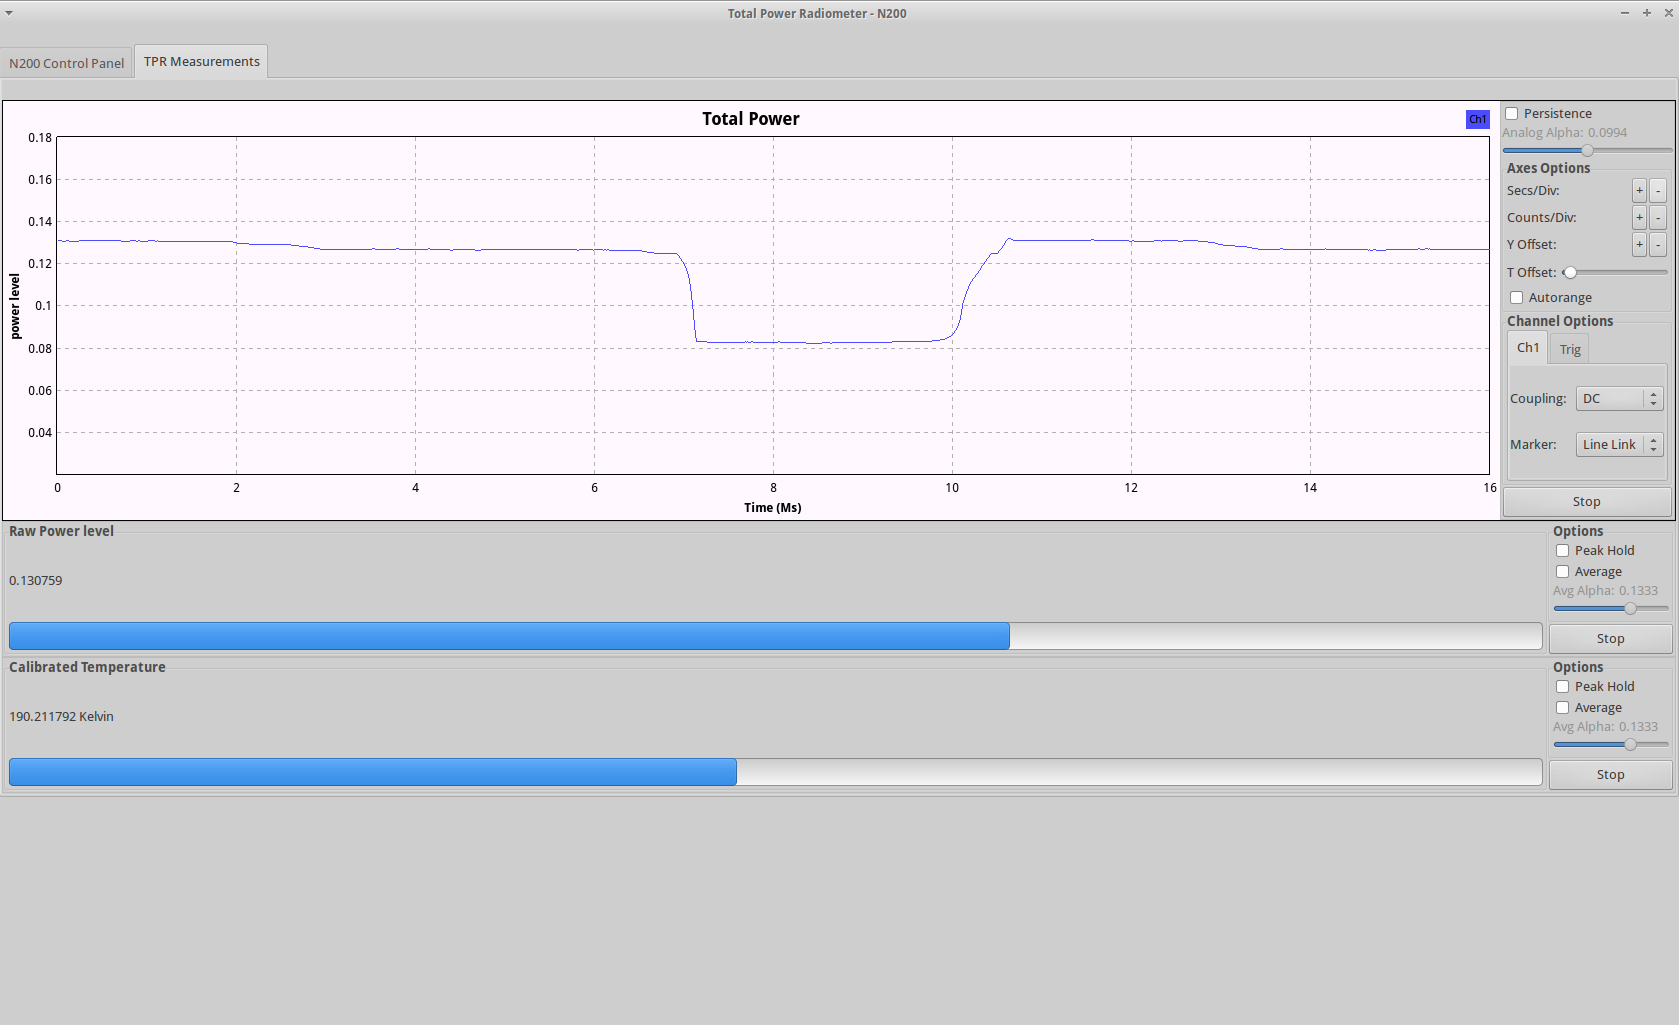
\includegraphics[width=17cm]{Images/Lab1_TPR_at_end_exp.png}
\isucaption{A screenshot showing the ticker tape display for the total power readings.  In addition, raw and calibrated noise temperature is shown below.}
\label{radiometer_tpr_display}
\end{figure}
}

We are not limited to just total power from the radiometer.  If the radiometer has been calibrated, those calibration points can be entered and GNURadio can calculate the calibrated noise temperature.  Additional information may also be added as needed.  For example, we are able to view the full spectrum that the radiometer sees.  This can be a useful tool for looking at potential RFI issues.  
%----------------------------------------------------------------------------------
%Everything below this needs to be moved/shifted or deleted

%\section{Square-law Detector Performance}
%The Square-law detector was added to our system in order to give us another reference point and to help verify the power output that the software defined radio.  Performance of our square-law detector is based on two items; the sensitivity of the diode used in the square-law detector and the analog to digital converter used to convert the analog voltage to a digital value.  The sensitivity of this device accounts for most of the performance factor of the system.  In our system the output of this square-law detector is then feed directly into an analog to digital converter.  Therefore, the performance of this A/D converter needs to be accounted for as well [\cite{Terlep}].  

%For our square-law detector, it has a noise output of $25nV/ \sqrt{Hz}$ at 100 kHz and will detect a signal as low as $-60$ dBm.  This works will with our needs since the RF front end brings the noise floor to approximately $-30$ dBm.
